%!TEX root = ../thesis.tex

本章では，報酬関数の変化が歩行動作へ与える影響を調査するために行う実験条件と評価指標について述べる．
\section{実験方法}
第3章の0節で，報酬関数とそのパラメータについて述べた．本研究では，それらをパラメータを変化させる基準として実験を行う．
以下に調査の対象とする報酬関数とその比較をするパラメータを示す．

\section{評価指標}
以下の論文を参考に，各報酬関数のパラメータを変更させて実験を行い，歩行動作に与える影響を評価する．
以下は，評価指標の一覧である．
\begin{itemize}
  \item 各関節のトルク，速度
  \item 歩行速度前進$1[m/s]$に対する追従率
  \item 床反力
  \item 胴体の姿勢のズレ
  \item 左右の歩幅
  \item 重心と左右の足上げ高さ
  \item CoT（Cost of Transport）
\end{itemize}

\section{評価指標に則り標準パラメータで学習した結果}

\begin{figure}[H]
  \centering
 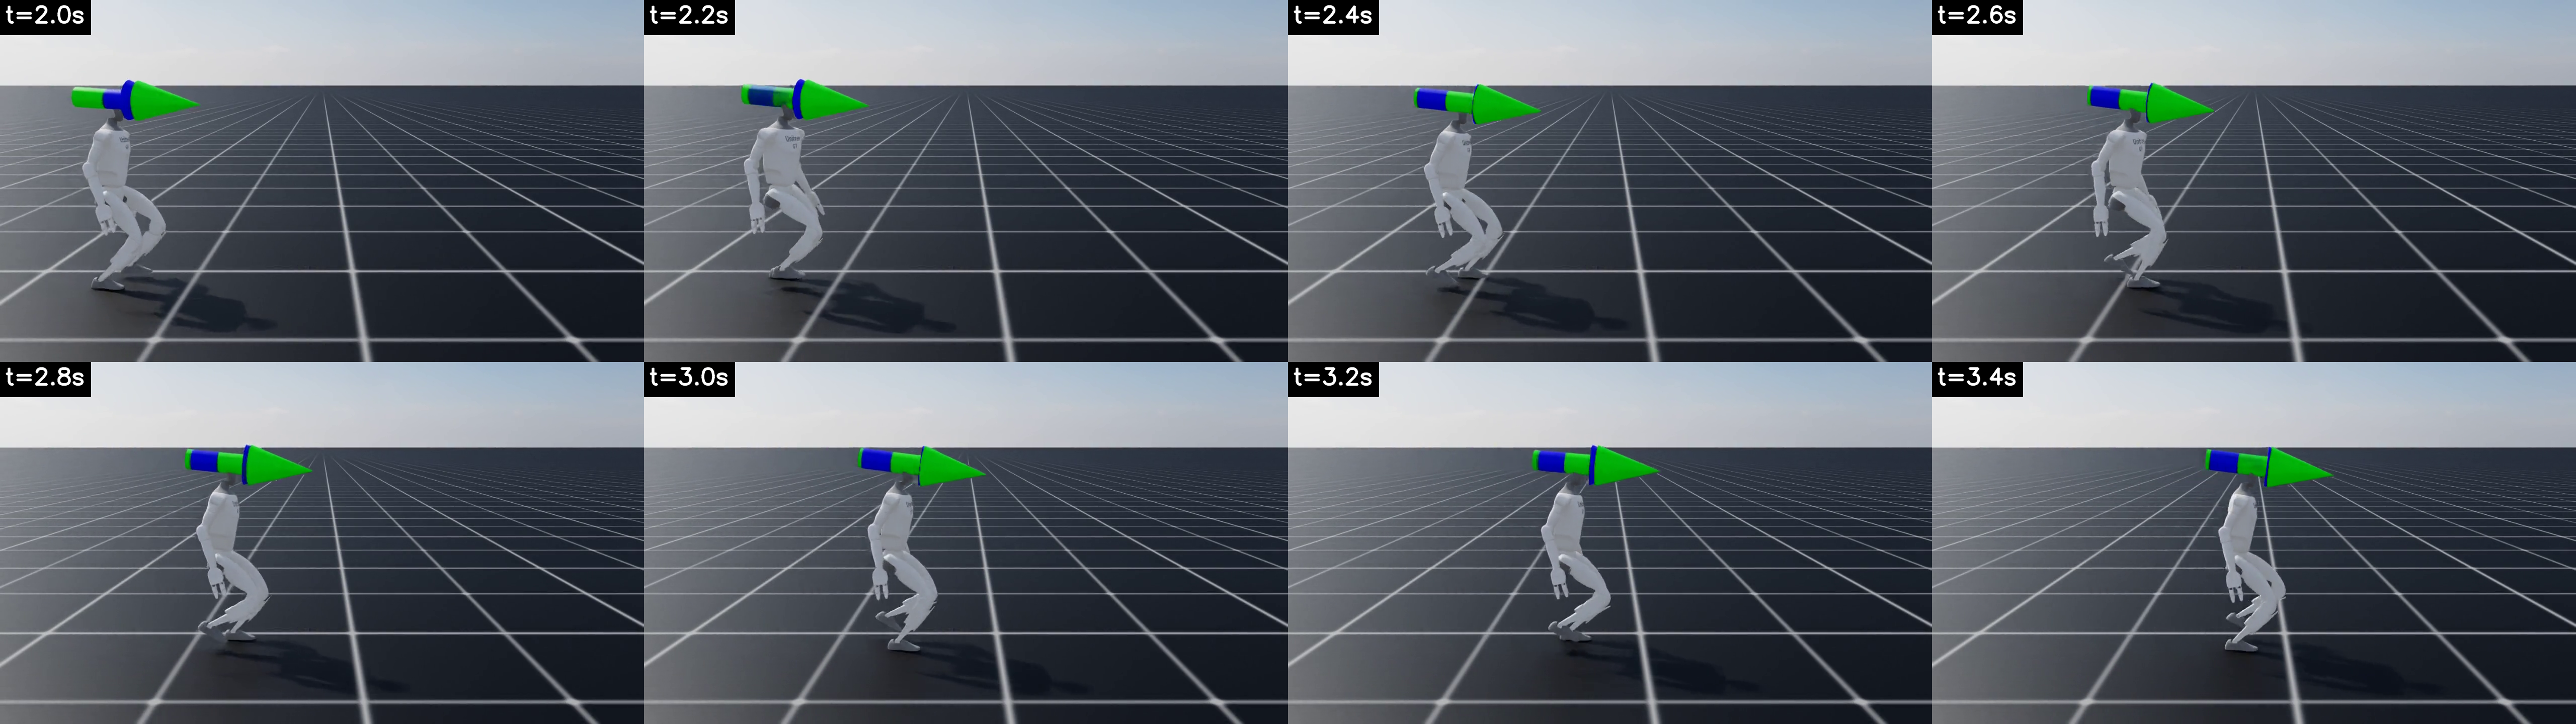
\includegraphics[keepaspectratio, scale=0.08]
      {images/png/sequence_final.png}
 \caption{Walking behavior with standard parameters}
 \label{Fig:Walking behavior with standard parameters}
\end{figure}

% 評価指標に則りFlat環境のデフォルトパラメータで学習した結果をプロットした図
\begin{figure}[H]
\centering
\begin{minipage}[b]{0.49\columnwidth}
    \centering
    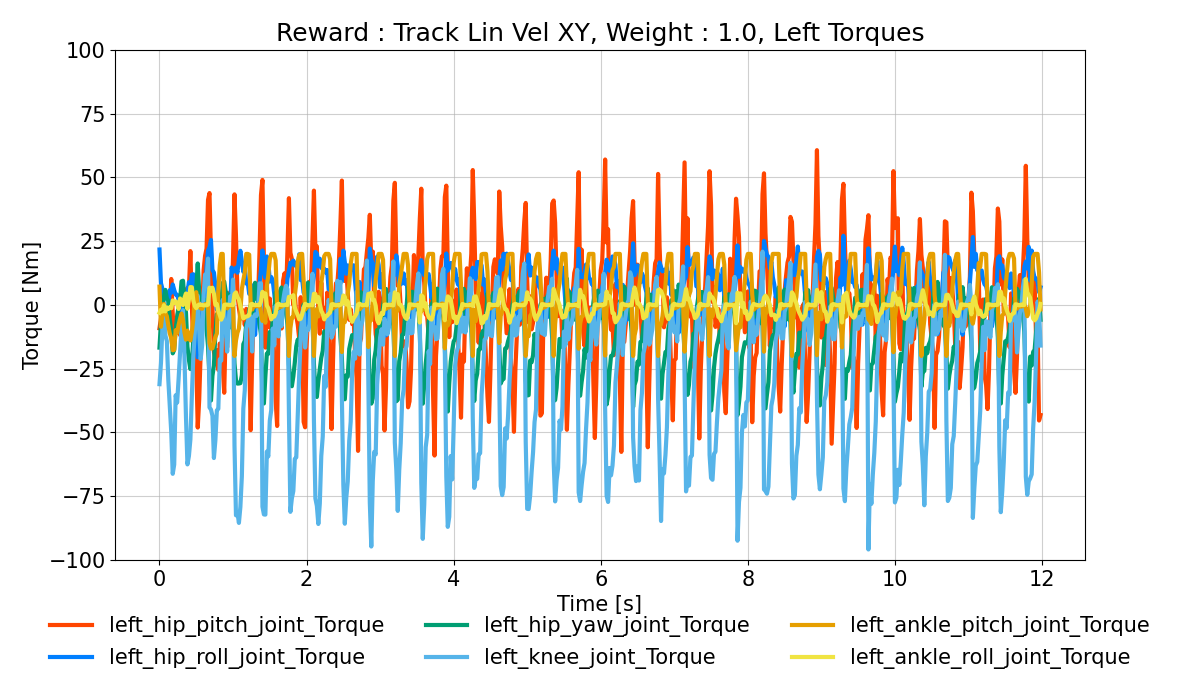
\includegraphics[width=1.0\columnwidth]{images/g1_flat_track_lin_vel_xy_exp/10/Left_Torques.png}
\end{minipage}
\begin{minipage}[b]{0.49\columnwidth}
    \centering
    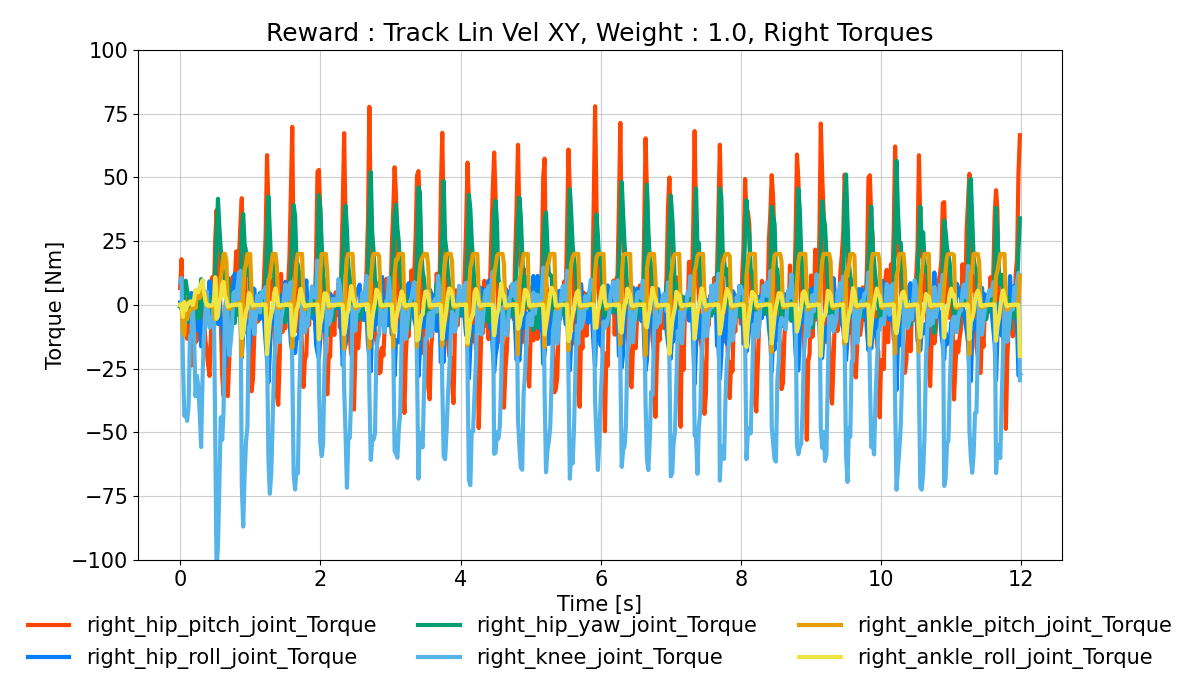
\includegraphics[width=1.0\columnwidth]{images/g1_flat_track_lin_vel_xy_exp/10/Right_Torques.png}
\end{minipage}
\end{figure}

\begin{figure}[H]
\centering
\begin{minipage}[b]{0.49\columnwidth}
    \centering
    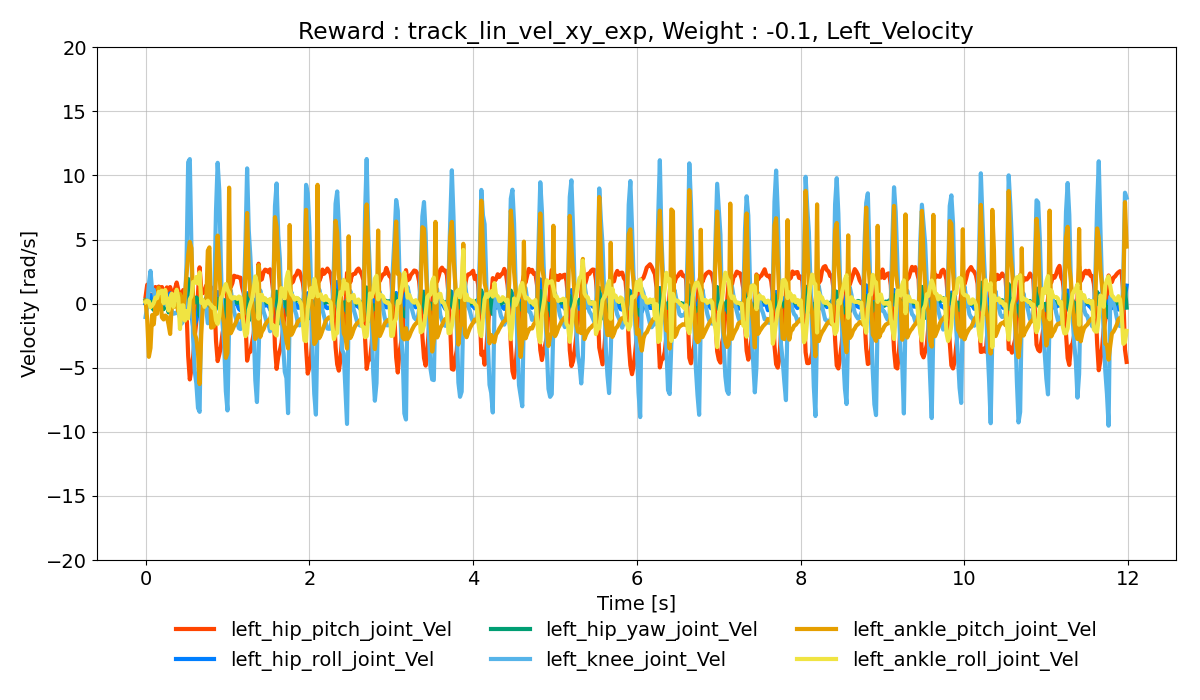
\includegraphics[width=1.0\columnwidth]{images/g1_flat_track_lin_vel_xy_exp/10/Left_Velocity.png}
\end{minipage}
\begin{minipage}[b]{0.49\columnwidth}
    \centering
    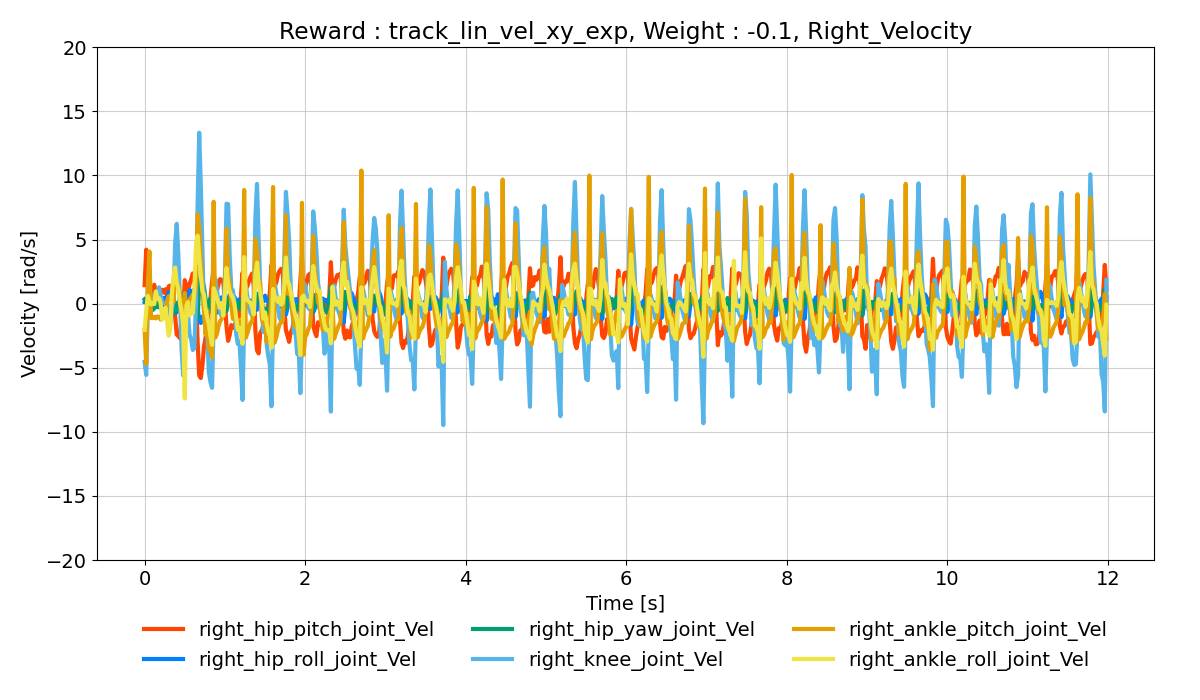
\includegraphics[width=1.0\columnwidth]{images/g1_flat_track_lin_vel_xy_exp/10/Right_Velocity.png}
\end{minipage}
\end{figure}

\begin{figure}[H]
\centering
\begin{minipage}[b]{0.49\columnwidth}
    \centering
    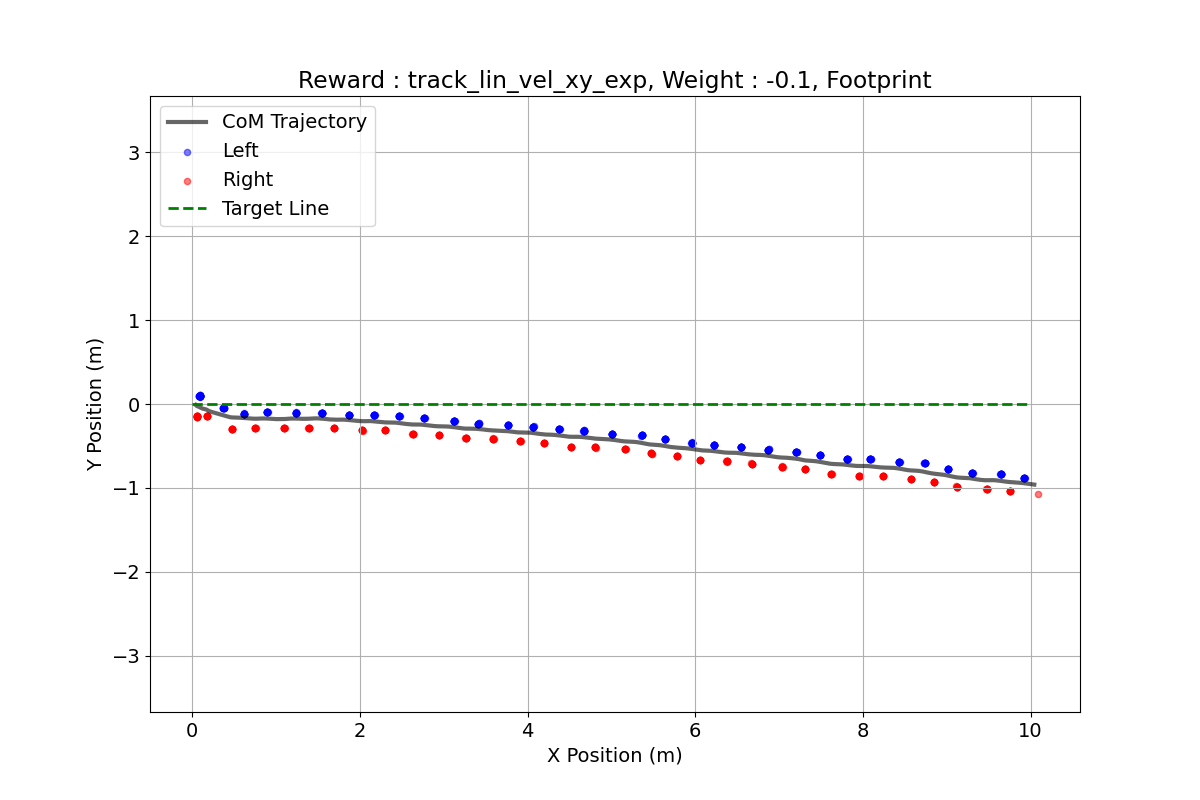
\includegraphics[width=1.0\columnwidth]{images/g1_flat_track_lin_vel_xy_exp/10/footprint_2d.png}
\end{minipage}
\begin{minipage}[b]{0.49\columnwidth}
    \centering
    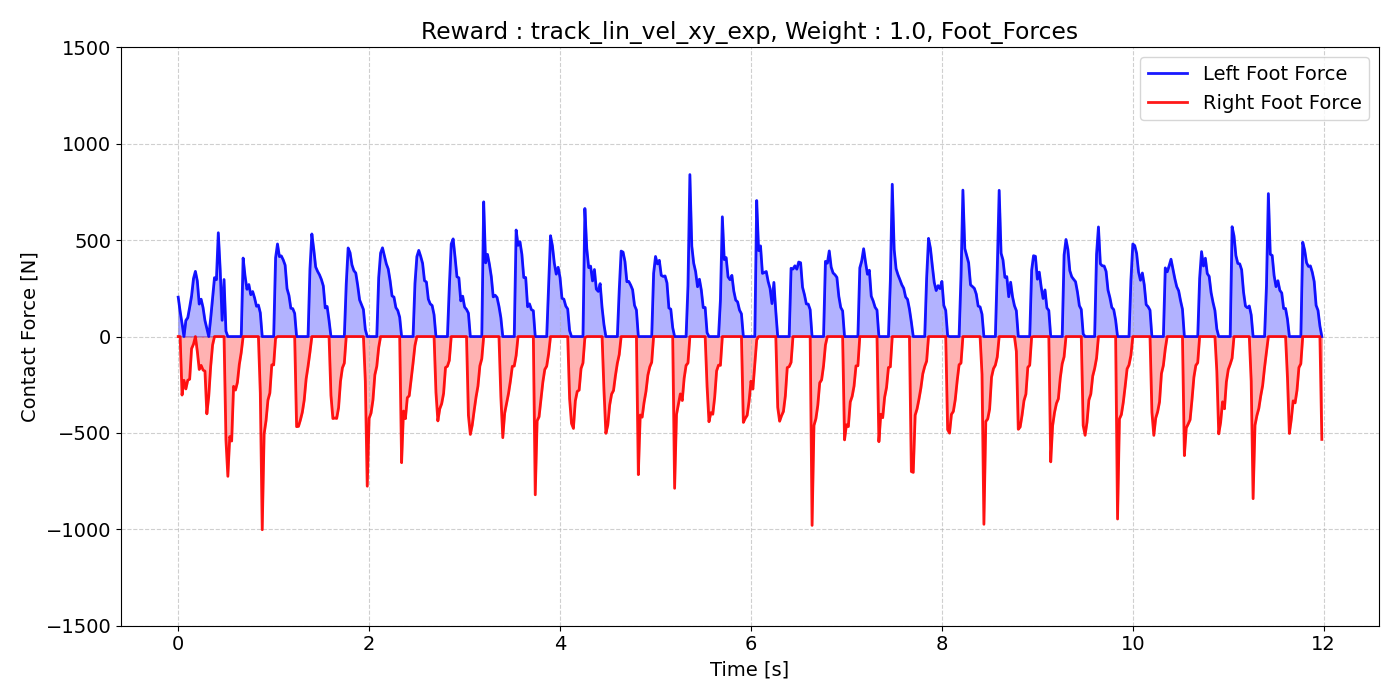
\includegraphics[width=1.0\columnwidth]{images/g1_flat_track_lin_vel_xy_exp/10/foot_force_plot.png}
\end{minipage}
\end{figure}

\begin{figure}[H]
\centering
\begin{minipage}[b]{0.47\columnwidth}
    \centering
    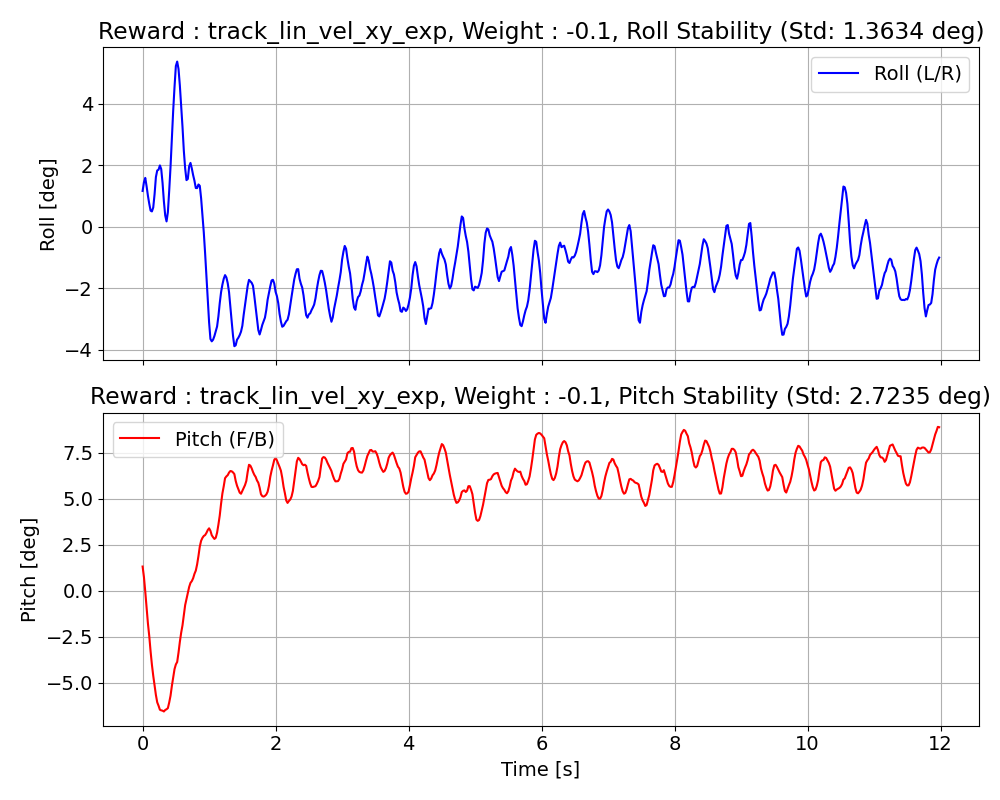
\includegraphics[width=0.9\columnwidth]{images/g1_flat_track_lin_vel_xy_exp/10/stability_analysis.png}
    \vfill
    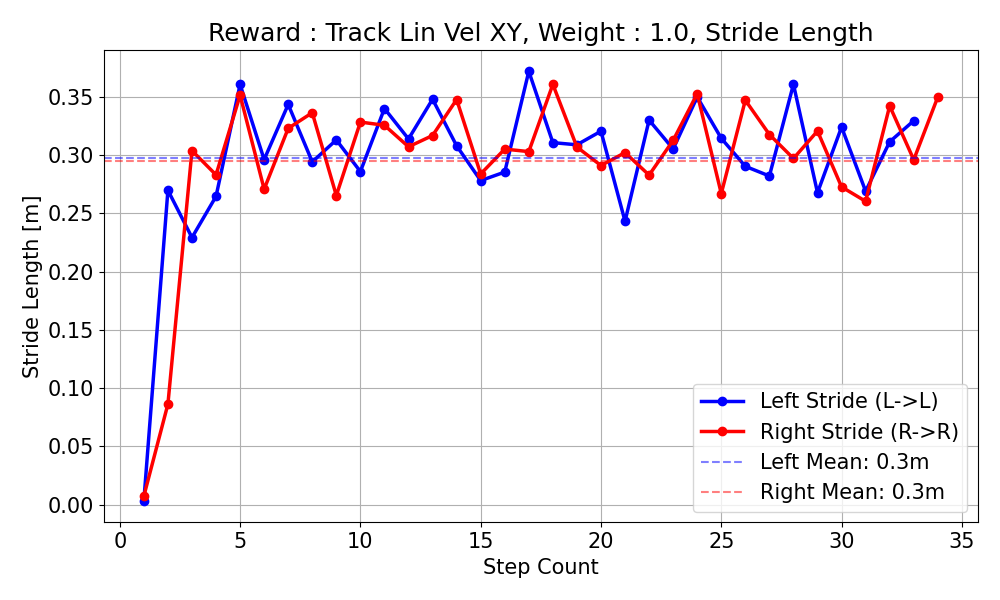
\includegraphics[width=0.9\columnwidth]{images/g1_flat_track_lin_vel_xy_exp/10/stride_length_analysis.png}
\end{minipage}
\begin{minipage}[b]{0.51\columnwidth}
    \centering
    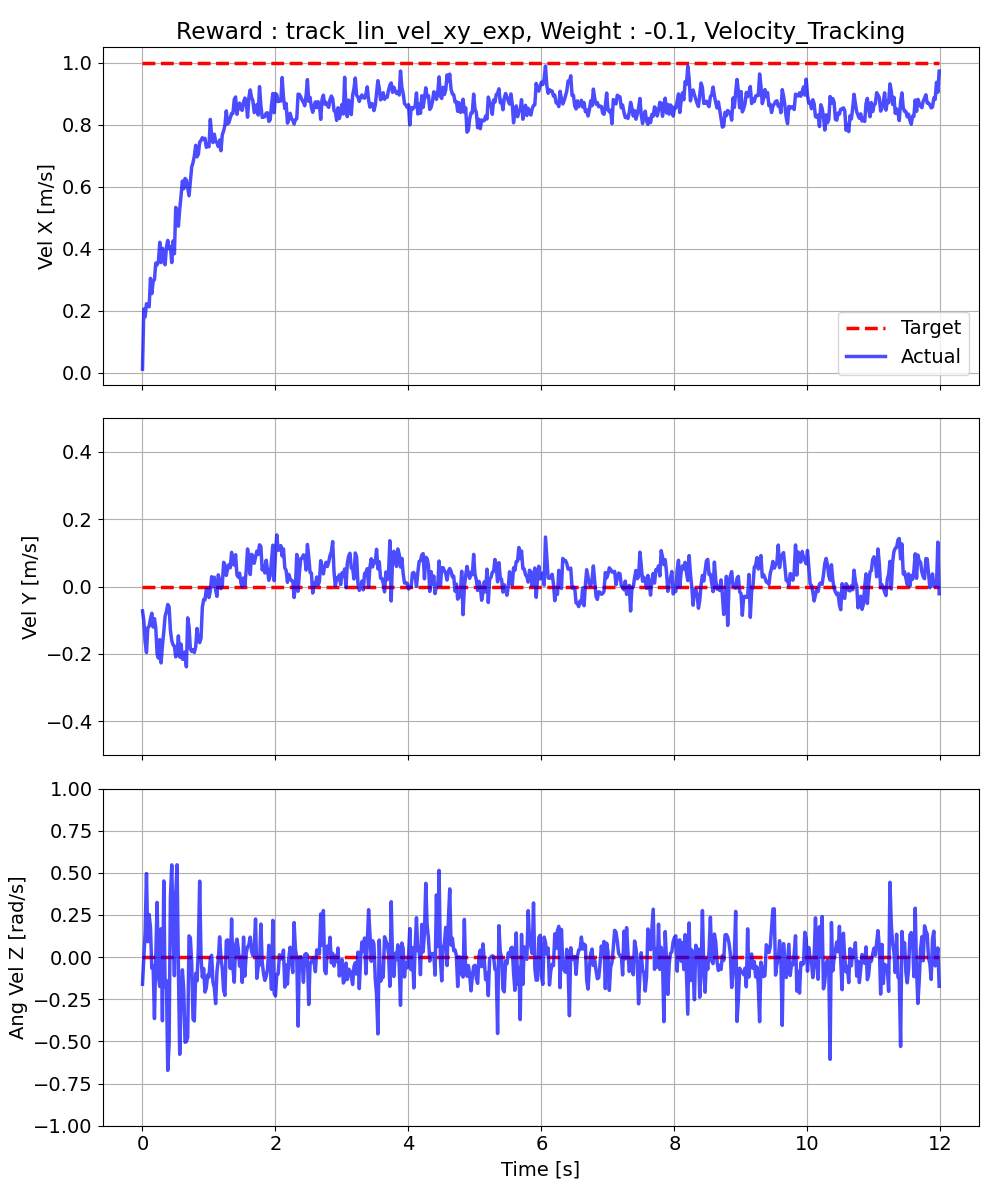
\includegraphics[width=0.9\columnwidth]{images/g1_flat_track_lin_vel_xy_exp/10/velocity_tracking.png}
\end{minipage}
\end{figure}

\begin{figure}[H]
  \centering
 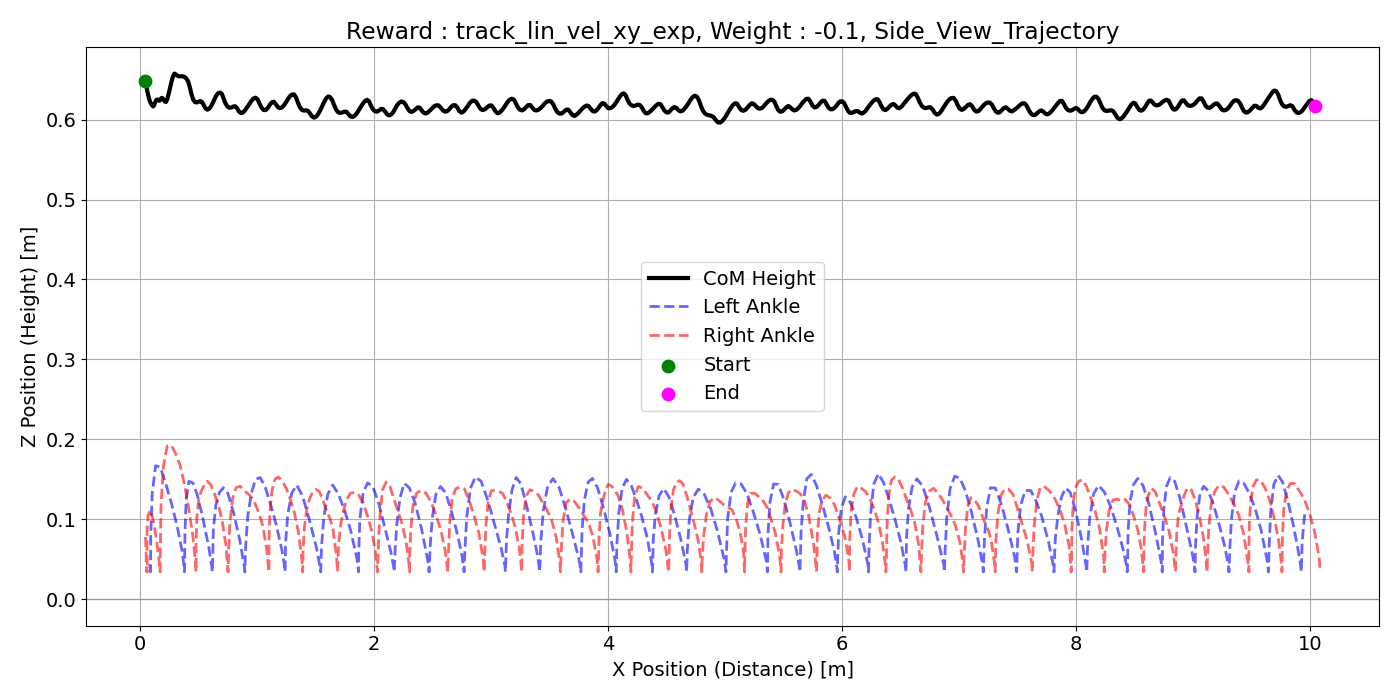
\includegraphics[keepaspectratio, scale=0.3]
      {images/g1_flat_track_lin_vel_xy_exp/10/trajectory_side_view.png}
\end{figure}

\newpage
